%\documentclass{article}
%\usepackage[utf8]{inputenc}
%\usepackage{amsmath}
%\usepackage{natbib}
%\usepackage{graphicx}
%\usepackage{astrojournals} % Necesario para nombres de revistas en luis-ref.bib
%\usepackage[spanish, es-minimal]{babel}
%\usepackage{longtable}
%\usepackage{geometry}
%\usepackage{multirow, array}
%\newlength\figwidth
%\setlength\figwidth{0.48\textwidth}
%\bibliographystyle{apj}


%\title{Catalog of stationary bowshock arcs in the Orion Nebula}

%\author{
  %Alumno: Luis Angel Gutiérrez Soto\\
  %Tutor: Dr. William Henney
%}
%\begin{document}
%\maketitle

%\section{Metodología}
\label{chap:methodology}
Detectamos todos los arcos de emisión estacionarios (objetos LL y y choques de proa asociados a proplyds) en unas imágenes del \textit{HST} de la Nebulosa de Orión. Se hizo la caracterización de los objetos LL es decir, se medieron los radios característicos (\(R_{c}\) y \( R_{0}\)), se estimó  la distancia \(D\) de la fuente a \thC{}, se determinó la anchura \(h\) de la cáscara y se  midieron  los valores de la emisión en las imágenes del ACS y WFPC2, para ello determinamos la forma de los arcos de los choques estacionarios, usando las herramientas del programa ds9 SAO image y con ello las imágenes de \citet{Bally:2006a}, en las cuales previamente habíamos identificamos los ya mencionados objetos de este estudio. Después de haber obtenido los valores de las imágenes se hicieron la pertinentes calibraciones del flujo en las mismas.

\section{Formas de los arcos}
\label{sec:arcos}

Una vez que se han identificado los todos proplyds y objetos LL en las imágenes tomadas por la cámara WFC-ACS usando el filtro de banda ancha F658N, se procedió a determinar la forma de los arcos de los choques estacionarios, usando estas mismas imágenes y las herramientas computacionales de ds9 SAO image. En este orden de ideas trazamos las posiciones de las estrellas jóvenes y de la misma manera las posiciones de los arcos (ver figura \ref{fig:arco-LL1}). Para ello en las imágenes FITS  establecimos las posiciones de las estrellas usando pequeños círculos. Para delimitar el borde externo del choque y desde luego determinar las coordenadas del mismo se usaron ``x'' y  para trazar el borde interno se usaron ``cruses (+)'', como se logra ver en la figura \ref{fig:arco-LL1} y es así como trazamos y medimos las coordenadas de la  región que comprende el choque y la posicion de la estrella central. 

\begin{figure}
  \centering
   \includegraphics[width=.6\linewidth]{figuras-tesis/forma-LL1.jpg}
  \caption{Formas de los arcos para LL1. Donde los bordes de los choques (externo e interno) están delimitados por los puntos (``x'' y ``+''). Esta imagen es tomada del campo 01 de \citet{Bally:2006a} (ACS-F658N) en el sur-oeste de la Nebulosa de Orión, por tanto es una imagen de \ha{}+\nii{}. }
  \label{fig:arco-LL1}
\end{figure}

\section{Estimación de los parámetros. \(D\), \(R_{0}\) , \(R_{c}\) y \(h_{0}\) }
\label{sec:parametros}

El propósito de trazar los arcos hiperbólicos radica en  que con esta información (coordenadas) fue posible estimar varios parámetros observacionales, que nos permitieran extraer información acerca de los choques. En este orden de ideas, una vez que ya teníamos las posiciones tanto de las componentes de los choques como de la estrella misma se pudo establecer la distancia \(D\), desde la fuente a \thC{} esta medida nos resultará muy útil como vermos más adelante. De la misma manera se midió \(R_{0}\), este radio lo vamos a definir como la distancia a lo largo del eje de simetría, de la fuente\footnote{La fuente podría ser una estrella T-Taury o un proplyd. Objetos de los cuales se origina el viento interno.} \citep{Robberto:2005}  al borde externo o interno de la cáscara chocada, dependiendo de cual sea el caso. El eje de simetría es la línea proyectada en la dirección en que están orientados los arcos, en la figura \ref{fig:radios} y \ref{fig:anchura} está representada por la línea amarilla. No obstante, hay que aclarar que tenemos dos radios debido a la presencia de un borde externo e interno como ya se ha visto. \\ 

\begin{figure}[htp]
\centering
\begin{tabular}{l l}
(\textit{a}) & (\textit{b})  \\
  \includegraphics[width=0.45\linewidth, trim=40 0.98 40 50, clip]{./figuras-tesis/177-341-Bally-01-images-sin.jpg}&
 \includegraphics[width=0.45\linewidth, trim=40 0.98 40 50, clip]{./figuras-tesis/177-341-Bally-01-images.jpg}\\
\end{tabular}
\caption{(a) Proplyd 177-341 ubicado en el sureste de la Nebulosa de Orión. (b) Mismo proplyd con una representación de los radios caracterŕsticos: \(R_{0}(\Out{})\); que es el radio del choque externo, medido a lo largo del eje que va desde el proplyd a \(\theta^1\ \text{Ori}\ \text{C}\), este eje está representado por la línea amarilla. \(R_{c}(\Out{})\) y \(R_{c}(\In{})\); llamados radios de curvaturas, son los radios de los círculos ajustados a partir de los puntos (coordenadas) utilizadas para delimitar los bordes externo e interno de la cáscara chocada. }\label{fig:radios}
\end{figure}

Por otro la lado, se han determinado los radios de curvaturas \(R_{c}\), que en este sentido son los radios de los círculos que se han ajustado, utilizando los puntos con los cuales hemos trazado la forma de los choques (ver figura \ref{fig:radios}), en este sentido se han medido los radios de curvatura para el borde interno y el borde externo de la cáscara chocada y los hemos llamado; \(R_{c}(\Out{})\) y \(R_{c}(\In{})\) respectivamente. Es de notar que la posición de la estrella no corresponde con el centro de los dos círculos que hemos fijado, en otras palabras las posiciones de los centros de los círculos dependen de la forma de los arcos que hemos trazado, es así que estos radios (obtenidos a partir de los cículos ajustados) van a ser un indicador de que tan simétricos son los choques, puesto que como podemos ver en la figura \ref{fig:anchura}, el centro de los círculos no coincide con el eje, entonces estaríamos frente a un caso de un choque que no es rigurosamente simétrico.\\

Siguiendo con la metodología llevada a cabo, otro parámetro que hemos podido estimar ha sido la anchura \(h_{0}\), que como veremos va a ser muy importante para determinar características físicas de los choques. No obstante, \(h_{0}\) la  defineremos como el ancho de la cáscara chocada a lo largo del eje de simetría. Por tanto para determinar éste parámetro hemos hecho lo siguiente: a la distancia que se ha estimado desde el borde externo a la estrella o Proplyd (\(R_{0}(\Out{})\)) le hemos restado el radio del choque interno (\(R_{0}(\In{})\)) (ver figura \ref{fig:anchura}), en esta medida tendremos que la anchura está dada por \(h_{0} = R_{0}(\text{out}) - R_{0}(\text{in})\), que es desde luego también es estimado a lo largo del eje del objeto.

\begin{figure}[htp]
\centering
\begin{tabular}{l l}
(\textit{a}) & (\textit{b})  \\
  \includegraphics[width=0.45\linewidth, trim=40 0.98 30 10, clip]{./figuras-tesis/042-628-Bally_16-images.jpg}&
 \includegraphics[width=0.45\linewidth, trim=40 0.98 30 10, clip]{./figuras-tesis/042-628-Bally_16-images-radii.jpg}\\
\end{tabular}
\caption{(a) Proplyd 042-628 y su respectivo choque de proa. (b) En esta imagen se puede apreciar el mismo proplyd 042-628  con una representación de la anchura \(h_{0}\) y del radio del choque interno \(R_{0}\) a lo largo del eje proplyd-estrella ionizadora. El eje está representado por la línea amarilla.  }\label{fig:anchura}
\end{figure}


\section{Estimación y calibración final del flujo-líneas de emisión en las imágenes del ACS y WFPC2}
\label{sec:clibration-final}

\subsection{Determinación de los valores  de la emisión en las imágenes del ACS y WFPC2 }
\label{sec:brillo-superficial}
Otras de las cosas que hemos realizado con nuestros objetos de estudios, ha  sido determinar el brillo superficial de cada uno de ellos. Una vez que hemos trazado la forma de los arcos hiperbólicos, se han extraído de los campos de Bally (que cubren en su mayoría a la Nebulosa de Orión), pequeñas imágenes FITS que sólo abarcan las regiones donde se encuentran los objetos LL y los proplyds, con el propósito de facilitar las mediciones de los valores de las imágenes. Esto mismo se hizo con los campos de Robberto. Así que usando estás pequeñas imágenes hemos medido los valores de las imágenes\footnote{En el caso de de las campos de Bally los valores de las imágenes tienen unidades de \(\mathrm{electrones~s^{-1}}\) y en caso de las imágenes de Robberto tienen unidades de \(\text{counts}~\text{s}^{-1}\).} en un determinado número de puntos o pixeles a lo largo de diferentes ángulos \(\theta\) en la región chocada y en el fondo, donde se ha supuesto que \(\theta = 0\) corresponde al eje proyectado en el plano del cielo que sigue la dirección en que llegan los fotones ionizantes provenientes de la estrella masiva y todos los demás ángulos \(\theta\) se forman a partir de dicho eje, en sentido contrario a las manesillas del reloj. Para ser más didácticos miremos un caso particular de los resultados de tales mediciones, es así que la figura \ref{fig:brillo-theta} nos muestra los valores en función de \(\theta\) para LL1, no obstante es de notar que esta gráfica permite ver los valores en el fondo, en la zona chocada y más rigurosamente en el centro de la cáscara. Estas mediciones se hicieron tomando la imágenes de la cámara ACS-F658N y de la misma manera se procedió con las imágenes de WFPC2-F656N \citep{Robberto:2013a}. \\

\begin{figure}[htp]
\centering
\begin{tabular}{l l}
(\textit{a}) & (\textit{b})  \\
  \includegraphics[width=0.5\linewidth, trim=60 10 70 50, clip]{./j8oc01010_wcs/w005-514-Bally_01-arcbright-th.jpg}
& \includegraphics[width=0.5\linewidth, trim=60 10 70 50, clip]{./j8oc01010_wcs/w005-514-Robberto_WFPC2_27_f656n-arcbright-th.jpg}\\
\end{tabular}
\caption{Valores del brillo superficial para el proplyd w005-514 en unidades de [\(\text{electrones}~\text{s}^{-1}\)], en función de los ángulos theta. Para (a) WCS F658N (b) WFPC2 F656N.}\label{fig:brillo-theta}
\end{figure}


Por otro lado también se determinó los valores del brillo superficial en función de la posición con respecto a los arcos, dicha posición se ha escrito de la siguiente forma; \(z = (R - R_{\text{in}})/(R_{\text{out}} - R_{\text{in}})\), que serían los radios relativos a la cáscara, donde \(R\) es la separación radial, \(R_{\text{in}}\) es el radio  desde la estrella al borde externo y \(R_{\text{in}}\) es el radio desde  la estrella al borde interno, es así que la figura \ref{fig:brillo-z} ilustra cuales son los valores para las diferentes radios relativos \(z\). Hay que resaltar que este tipo de gráficas las obtuvimos para cada uno de los choques estacionarios.\\

\begin{figure}[htp]
\centering
\begin{tabular}{l l}
(a) & (b)  \\
  \includegraphics[width=0.5\linewidth, trim=60 10 70 50, clip]{./j8oc01010_wcs/w005-514-Bally_01-arcbright-z.jpg}
& \includegraphics[width=0.5\linewidth, trim=60 10 70 50, clip]{./j8oc01010_wcs/w005-514-Robberto_WFPC2_27_f656n-arcbright-z.jpg}\\
\end{tabular}
\caption{Valores del brillo superficial para el proplyd w005-514 en función de la posición  \(z = (R - R_{\text{in}})/(R_{\text{out}} - R_{\text{in}})\). Para (a) WCS F658N (b) WFPC2 F656N.}\label{fig:brillo-z}
\end{figure}

Dado que se tenían los valores de la emisión de los pixeles para las diferentes zonas de los choques hiperbólicos como se mencionó arriba, entonces como siguiente paso se determinaron los valores promedios en la cáscara chocada, en el fondo y en el centro de la cáscara. Hay que tener en cuenta que los valores determinados para las cáscara incluyen los del fondo, entonces para tener unos valores coherentes del mismo, es decir sólo de la cáscara, le hemos restado los valores del fondo. Es importante mencionar que de la misma manera hemos medido los valores de la emisión de las  imágenes de los viejos  mosaicos de WFPC2, es decir aquellas  observaciones obtenidas con el uso de los filtros F656N (\(\mathrm{\ha~6563~\A{}}\)), F658N (\(\mathrm{\nii~6583~\A{}}\)), f502n (\(\oiii{}~5007~\A{}\)) y del filtro para el continuo f547m.\\

\subsection{Estimación de las constantes de calibración}
\label{sec:const}
En esta parte del trabajo hemos escrito los valores de las emisiones medidos en las observaciones de las respectivas cámaras, en unidades físicas esto es en [\(\mathrm{erg\ s^{-1}\ cm^{-2}\ sr^{-1}}\)]. Como ya se dijo los valores medidos en las imágenes tomadas por la cámara ACS con el fitro F658N tienen unidades de [\(\mathrm{electrones\ s^{-1}}\)] y las unidades de los valores en las imágenes de WFPC2 con el filtro F656N tienen unidades de [\(\text{counts}\ \text{s}^{-1}\)], entonces se relizó la respectiva conversión de unidades con el propósito de tener el brillo superficial obtenidos apartir de las imágenes de las cámaras ACS y WFPC2 en las mismas unidades físicas.\\


\subsubsection{Estimación de las constantes de calibración de las imágenes de Bally (ACS-F658N) y Robberto (WFPC-F656N)}
\label{sec:acs}

Para la estimación de los coeficientes de calibración obtuvimos la información clave para la fotometría, del encabesado de las imágenes FITS a través de ds9. Primero determinamos esta constante de calibración para las imágenes de la cámara ACS con el filtro F658N. Entonces como se mencionó  en la sección~\ref{sec:brillo-superficial} las imágenes están en unidades de [\(\mathrm{electrones\ s^{-1}}\)], es así que si se multiplican por el PHOTFLAM (inverse sensitivity) que aparece en el encabezado y cuyas unidades están en [\(\mathrm{erg\ cm^{2}\ \AA{}\ electrones}\)], se obtienen unidades de [\(\mathrm{erg\ s^{-1}\ cm^{2}\ \AA{}\ pixel^{-1}}\)]. No obstante al multiplicar por la anchura rectangular del filtro nos libramos del término \A{} y al dividir por el área del pixel, información que también se obtuvo del encabezado. Vemos que se pueden escribir los valores de las imágenes en unidades de brillo superficial [\(\mathrm{erg~s^{-1}~cm^{-2}~ sr^{-1}}\)], esta constante es presentada en la tabla~\ref{tab:table-constans}. Para determinar la anchura del filtro se usó una paquetería de python llamada ``pysynphot'', al implementarse esta mostró que la anchura rectangular es 74.9405 \(\text{\AA{}}\), esto se hizo separadamente porque esta información no está incluida en el encabezado de las imágenes FITS\\

En segundo lugar se determinó el coeficiente de calibración  para las imágenes de \citet{Robberto:2013a} (WFPC2-F656N). Esto se hizo usando el mismo procedimiento descrito arriba (calibración del brillo en las imágenes de Bally), para escribir en unidades de brillo superficial los valores de la emisión \(\ha{}~6563~\A{}\) de estas imágenes. Aunque es de notar que para este caso se obtuvo para la anchura del filtro un valor de 28.34207~\A{}. El coeficiente de calibración resultante se puede ver en la tabla~\ref{tab:table-constans}.\\

\subsubsection{Estimación de las  constantes de calibración de las imágenes de los mosaicos de WFPC2}
\label{sec:wpfc2}
Las imágenes del mosaico de WFPC2 para el filtro F656N (\(\mathrm{\ha~6563~\AA{}}\)) y el filtro F658N (\(\mathrm{\nii~6583~\AA{}}\)) están unidades de [counts], así que para obtener unidades de brillo superficial, también se estimó un coeficinete de calibración para estas observaciones. Para determinar dichas constantes de calibración se hizo el siguiente análisis; para obtener unidades de \(\mathrm{count~s^{-1}}\) hay que  dividir entre el tiempo de exposicón, teniendo en cuenta que las observaciones tomadas con el filtro F656N tiene un tiempo de exposición de 200~s y las del filtro F658N tiene un tiempo de exposición de 500~s. Ahora, si estos valores en unidades de [\(\mathrm{count~s^{-1}}\)], se dividen entre los coeficientes de calibración de \citet{Odell:2009}, los cuales a llamado \(\mathrm{K1_{fiter}}\) respectivamente son: \(\mathrm{K1_{F656N} = 1.62}\) y \(\mathrm{K1_{F658N} = 160}\) con unidades de [\(\mathrm{10^{-10}~counts~cm^{2}~sr~phtons^{-1}}\)], se obtienen unidades de [\(\mathrm{photons~s^{-1}~cm^{-2}~sr^{-1}}\)]. Por último, al multiplicar por la energía del fotón (\(\mathrm{E=3.027\times 10^{-12}~erg~para~\ha{}~6563~\AA{}}\) y \(\mathrm{E=3.018 \times10^{-12}~erg}\) para \(\nii{}~6583~\A{}\)) se obtienen cantidades con unidades de 
[\(\mathrm{erg~s^{-1}}\)  \(\mathrm{cm^{-2}~sr^{-1}}\)] que al final de cuentas es lo que se quiere.  Con este análisis concluimos que al realizar la operación \(1/(\mathrm{TK1_{fiter}E}\))  podemos obtener las cosntantes de calibración deseadas, donde T es el tiempo de exposición y E la energía del fotón. En la tabla~\ref{tab:table-constans} se pueden apreciar los valores de los coeficientes para F656N y F658N. 


\begin{table}[htp]
\centering
\small\raggedright
\renewcommand{\arraystretch}{1.5}
\caption{Valores de los coeficientes de calibración.}
  \label{tab:table-constans}

\begin{tabular}{ |l| |c| |l| }
\hline
Cámara-filtro&                       Coeficiente de calibración&       Unidades\\ \hline 
ACS-F658N (Imágenes de Bally)&       0.00250 &                          \(\mathrm{erg~electrones^{-1}~cm^{-2}~sr^{-1}}\)\\
WFPC2-F656N (Imágenes de Robberto)&  0.16896 &                          \(\mathrm{erg~counts^{-1}~cm^{-2}~sr^{-1}}\)\\
WFPC2-F656N (Mosaico)&               0.00009 &                          \(\mathrm{erg~counts^{-1}~s^{-1}~cm^{-2}~sr^{-1}}\)\\
WFPC2-F658N (Mosaico)&               0.00004 &                          \(\mathrm{erg~counts^{-1}~s^{-1}~cm^{-2}~sr^{-1}}\)\\ 
\hline
 \end{tabular} 
 \end{table}
\normalsize

\subsection{Corrección por extinción}
\label{sec:extintion}

Una vez que se tenían los valores fotómetricos y calibrados en flujo, como siguiente paso se  realizó la corrección por extinción. Para ello se ha usado la extinción logarítmica: \(C = -\log(F'/F) = 0.4343\tau\) y  la extinción en magnitudes \(A=-2.5\log(F'/F)=2.5C=1086\tau\). Para la extinción nebular se ha escrito la extinción logarítmica como  \(C_{\lambda} = C_{\text{H}\beta}(A_{\lambda}/A_{\text{H}\beta})\). No obstante si  \(f_{\lambda}= E_{\lambda-\text{H}_{\beta}}/A_{\text{H}_{\beta}}=(A_{\lambda}/A_{\text{H}_{\beta}})-1\)  dado que \(E_{\lambda-\text{H}_{\beta}}=A_{\lambda}-A_{\text{H}_{\beta}}\), entonces se tiene que \(C_{\lambda}= C_{\text{H}\beta}(1+f_{\lambda})\)  de este modo  el flujo corregido por extinción es

\begin{equation}
  \label{eq:flujo}
  F_{\lambda} = F'_{\lambda}\times10^{C_{\text{H}\beta}(1+f_{\lambda})}
\end{equation}

 Donde  \(F_{\lambda}\) es el flujo intrínsico, \(F'_{\lambda}\) es el flujo observado. Para \(\ha\ 6563\text{\AA{}}\): \(f_{\lambda} = -0.220\) \citep{Blagrave:2007}. Es importante señalar que  apartir de un mapa de extinción de la Nebulosa de Orión hemos obtenido \(C_{\text{H}\beta}\).

\subsection{Comparación entre los brillos superficiales de WFPC2-F656N (\ha{}) y de ACS-F658N (\ha{}+\nii{})}
\label{sec:comp}

\begin{figure}
  \centering
   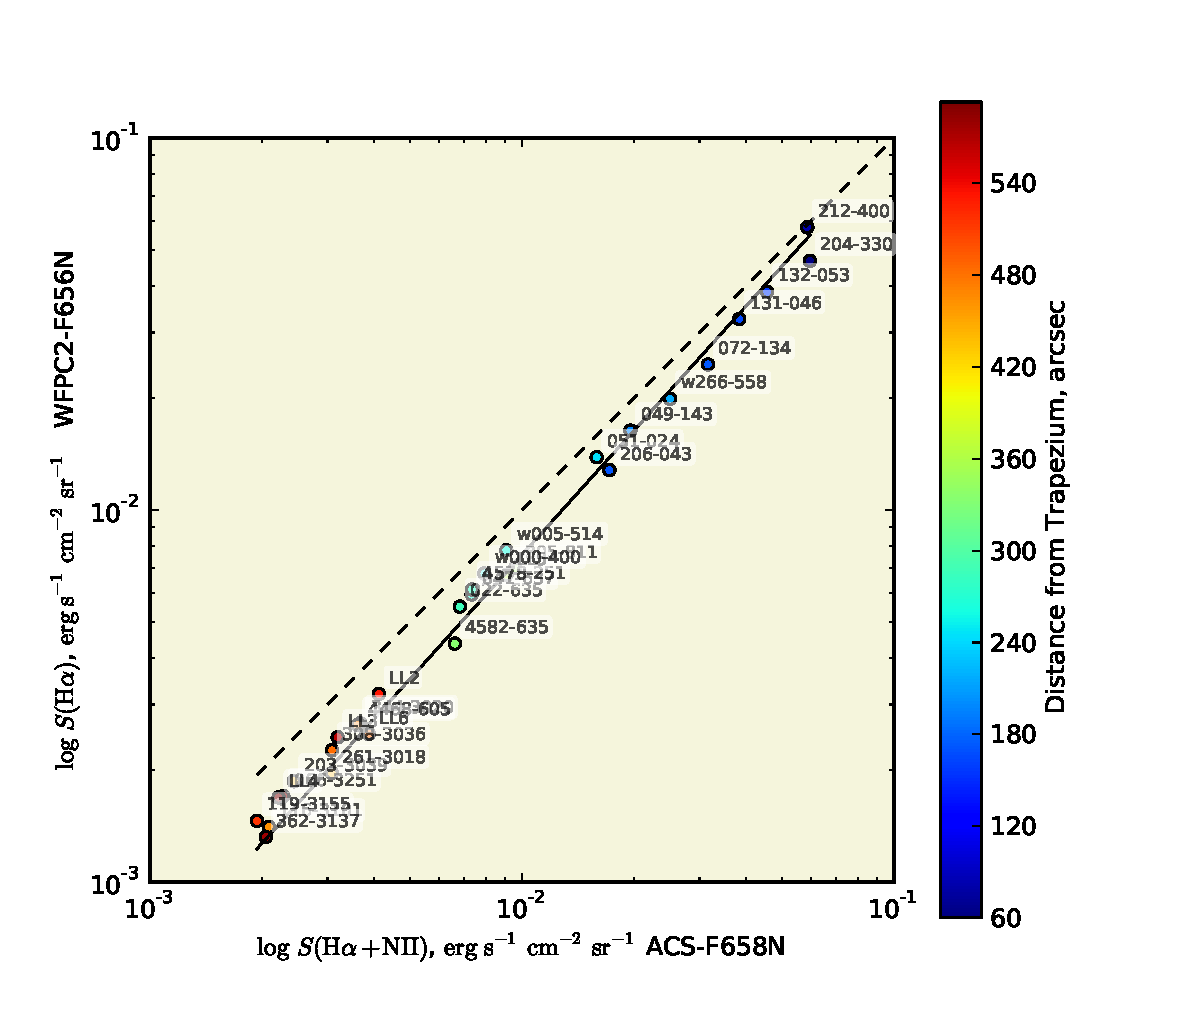
\includegraphics[width=0.9\linewidth, trim=20 20 30 50, clip]{luis-programas/S(alpha)_bg_WFPC2_ACS_calibrationlog-f.pdf}
  \caption{ Brillo superficial de \ha{} del fondo de nuestras muestras en las imágenes de Robberto (WFPC2-F656N) en función del brillo superficial de \ha{}+\nii{} las imágenes de Bally (ACS-F658N) en unidades  [\(\mathrm{erg\ s^{-1}\ cm^{-2}\ sr^{-1}}\)]. La línea continua indica un ajuste lineal de los puntos graficados, mientras que la línea discontinua representa una relación 1:1. La escala de colores indica la separación del Trapecio. }
  \label{fig:brillo-fisica}
\end{figure}

Ahora que habíamos hecho las calibraciones correspondientes del flujo, comparamos los resultados entre los brillos superficiales de las imágenes de ACS y WFPC2. La figura \ref{fig:brillo-fisica} nos muestra el tipo de relación que se da entre las valores de las dos imágenes de las respectivas cámaras, de donde podemos concluir que el brillo superficial de las observaciones de Bally para el fondo de cada uno de los objetos en las regiones externas de la nebulosa es un tanto mayor, si las comparamos con el brillo de las imágenes de WFPC2, esto sucede porque las imágenes de la camara ACS-F658N están contaminadas con las líneas de \(\nii{}\). Podemos decir que aproximadamnte el \(20\%\) del brillo superficial es la contribución de la emisión de \nii{} en estas regiones de la Nebulosa de Orión. Mientras que la contribución de la emisión de \nii{} en regiones cercanas del Trapecio es casi despreciable.\\

\subsection{Verificaciones de las calibraciones del brillo superficial para WFPC2}
\label{sec:verifi}


Una  forma utilizada para verificar que las calibraciones realizadas iban por buen camino, fue comparar nuestros resultados con  resultados ya publicados. En este sentido \citet{Henney:2013a} había determinado el brillo superficial para el frente de LL1, el cúal obtuvo un valor de \(0.02\ \mathrm{erg\ s^{-1}\ cm^{-2}\ sr^{-1}}\) después de hacer la corrección para una extinción de \(A(\ha{}) = 0.16 \pm 0.03\ \text{mag}\) de \ha{}. Usando la Ec. \ref{eq:flujo} determinamos que el brillo superficial observado es \(0.1726~\mathrm{erg\ s^{-1}\ cm^{-2}\ sr^{-1}}\) y dado que el valor de la emisión (count rate) para la imagen de LL1 de la cámara WFPC2 es de 0.10 count, entonces encontramos que el factor de calibración usada para el ajuste del flujo en dicho artículo fue de  0.1726. Esta constante de calibración es muy similar a la obtenida por nosotros usando el método de la sección \S\ref{sec:const} (ver tabla~\ref{tab:table-constans}).      

%\bibliography{luis-ref}

%\end{document}
